%%
%% This is file `sample-acmsmall-conf.tex',
%% generated with the docstrip utility.
%%
%% The original source files were:
%%
%% samples.dtx  (with options: `all,proceedings,bibtex,acmsmall-conf')
%% 
%% IMPORTANT NOTICE:
%% 
%% For the copyright see the source file.
%% 
%% Any modified versions of this file must be renamed
%% with new filenames distinct from sample-acmsmall-conf.tex.
%% 
%% For distribution of the original source see the terms
%% for copying and modification in the file samples.dtx.
%% 
%% This generated file may be distributed as long as the
%% original source files, as listed above, are part of the
%% same distribution. (The sources need not necessarily be
%% in the same archive or directory.)
%%
%%
%% Commands for TeXCount
%TC:macro \cite [option:text,text]
%TC:macro \citep [option:text,text]
%TC:macro \citet [option:text,text]
%TC:envir table 0 1
%TC:envir table* 0 1
%TC:envir tabular [ignore] word
%TC:envir displaymath 0 word
%TC:envir math 0 word
%TC:envir comment 0 0
%%
%% The first command in your LaTeX source must be the \documentclass
%% command.
%%
%% For submission and review of your manuscript please change the
%% command to \documentclass[manuscript, screen, review]{acmart}.
%%
%% When submitting camera ready or to TAPS, please change the command
%% to \documentclass[sigconf]{acmart} or whichever template is required
%% for your publication.
%%
%%
\documentclass[acmsmall]{acmart}
%%
\usepackage{enumitem}
\usepackage{graphicx}
\usepackage{subcaption}


%% \BibTeX command to typeset BibTeX logo in the docs
\AtBeginDocument{%
  \providecommand\BibTeX{{%
    Bib\TeX}}}

%% Rights management information.  This information is sent to you
%% when you complete the rights form.  These commands have SAMPLE
%% values in them; it is your responsibility as an author to replace
%% the commands and values with those provided to you when you
%% complete the rights form.
\setcopyright{acmlicensed}
\copyrightyear{2025}

\acmVolume{1}
\acmNumber{1}
\acmArticle{1}
\acmYear{2025}
\acmMonth{5}

\acmDOI{XXXXXXX.XXXXXXX}
%% These commands are for a PROCEEDINGS abstract or paper.
\acmConference[Conference '25]{Make sure to enter the correct
  conference title from your rights confirmation email}{June 03--05,
  2025}{Woodstock, NY}
%%
%%  Uncomment \acmBooktitle if the title of the proceedings is different
%%  from ``Proceedings of ...''!
%%
%%\acmBooktitle{Woodstock '18: ACM Symposium on Neural Gaze Detection,
%%  June 03--05, 2018, Woodstock, NY}

%%%%%%%%%%%%%%%%%%%%%%%%%%%%%%%%%%%%%%%%%
%\acmISBN{978-1-4503-XXXX-X/2018/06}


%%
%% Submission ID.
%% Use this when submitting an article to a sponsored event. You'll
%% receive a unique submission ID from the organizers
%% of the event, and this ID should be used as the parameter to this command.
%%\acmSubmissionID{123-A56-BU3}

%%
%% For managing citations, it is recommended to use bibliography
%% files in BibTeX format.
%%
%% You can then either use BibTeX with the ACM-Reference-Format style,
%% or BibLaTeX with the acmnumeric or acmauthoryear sytles, that include
%% support for advanced citation of software artefact from the
%% biblatex-software package, also separately available on CTAN.
%%
%% Look at the sample-*-biblatex.tex files for templates showcasing
%% the biblatex styles.
%%

%%
%% The majority of ACM publications use numbered citations and
%% references.  The command \citestyle{authoryear} switches to the
%% "author year" style.
%%
%% If you are preparing content for an event
%% sponsored by ACM SIGGRAPH, you must use the "author year" style of
%% citations and references.
%% Uncommenting
%% the next command will enable that style.
%%\citestyle{acmauthoryear}


%%
%% end of the preamble, start of the body of the document source.
\begin{document}

%%
%% The "title" command has an optional parameter,
%% allowing the author to define a "short title" to be used in page headers.
\title{Evaluating Recommender Systems for Digital Library Datasets}

%%
%% The "author" command and its associated commands are used to define
%% the authors and their affiliations.
%% Of note is the shared affiliation of the first two authors, and the
%% "authornote" and "authornotemark" commands
%% used to denote shared contribution to the research.

\author{Ákos Lévárdy}
%\authornote{Both authors contributed equally to this research.}
\email{levardyakos@gmail.com}
%\orcid{1234-5678-9012}
%\author{G.K.M. Tobin}
\authornotemark[1]
%\email{webmaster@marysville-ohio.com}
\affiliation{%
  \institution{Slovak Technical University}
  \city{Bratislava}
  \country{Slovakia}
}





%%
%% By default, the full list of authors will be used in the page
%% headers. Often, this list is too long, and will overlap
%% other information printed in the page headers. This command allows
%% the author to define a more concise list
%% of authors' names for this purpose.
%\renewcommand{\shortauthors}{Trovato et al.}

%%
%% The abstract is a short summary of the work to be presented in the
%% article.

%  A clear and well-documented \LaTeX\ document is presented as an
%  article formatted for publication by ACM in a conference proceedings
%  or journal publication. Based on the ``acmart'' document class, this
%  article presents and explains many of the common variations, as well
%  as many of the formatting elements an author may use in the
%  preparation of the documentation of their work.
%

%\begin{abstract}
%This work focuses on analysing and evaluating recommender systems best suitable for digital library datasets. With the rise of digital content, such systems help users navigate large information spaces by generating personalized recommendations. In the introduction we show the importance and role of Recommender Systems (RS) in filtering and anticipating user preferences across various domains. We then present an overview of the key recommendation techniques, explaining their underlying mechanisms and common challenges. The project emphasizes Content-Based Filtering techniques, comparing text representational methods like BERT, FastText, LSA, and TF-IDF. 
%Offline experiments were conducted to evaluate the system’s ability to generate Top-N book recommendations from the input data and the algorithms were compared based on evaluation metrics such as similarity, coverage, diversity or confidence. 
%The main objective of this work aims to design and implement a system capable of benchmarking different recommendation algorithms designed for digital library datasets and to provide insights into their effectiveness and applicability in this domain.
%\end{abstract}


\begin{abstract}
Recommender systems play a vital role in navigating the growing volume of digital content, especially in academic and digital library environments. This work presents a description of different recommendation methods and their chracteristics along with a comprehensive evaluation of the content-based recommender systems applied to book datasets. We compare seven text representation methods—TF-IDF, BoW, LSA, GloVe, FastText, BERT, and E5—through offline experiments using datasets composed of academic book paragraphs and Goodreads descriptions. The work describes the various evaluation metrics that are user for recommendation comparison. The evaluation on the tested algorithms and datasets includes similarity, coverage, diversity, and confidence. Our results highlight trade-offs in effectiveness and diversity across models. This paper provides actionable insights for selecting appropriate recommendation strategies for digital library use cases.
\end{abstract}

%%
%% The code below is generated by the tool at http://dl.acm.org/ccs.cfm.
%% Please copy and paste the code instead of the example below.
%%




\begin{CCSXML}
<ccs2012>
   <concept>
       <concept_id>10002951.10003260.10003282</concept_id>
       <concept_desc>Information systems~Content-based recommendation</concept_desc>
       <concept_significance>500</concept_significance>
   </concept>
   <concept>
       <concept_id>10010147.10010178.10010179.10010180</concept_id>
       <concept_desc>Computing methodologies~Natural language processing</concept_desc>
       <concept_significance>300</concept_significance>
   </concept>
   <concept>
       <concept_id>10010147.10010178.10010187</concept_id>
       <concept_desc>Computing methodologies~Learning latent representations</concept_desc>
       <concept_significance>300</concept_significance>
   </concept>
   <concept>
       <concept_id>10002951.10003260.10003310</concept_id>
       <concept_desc>Information systems~Evaluation of retrieval results</concept_desc>
       <concept_significance>300</concept_significance>
   </concept>
</ccs2012>
\end{CCSXML}

\ccsdesc[500]{Information systems~Content-based recommendation}
\ccsdesc[300]{Information systems~Evaluation of retrieval results}
\ccsdesc[300]{Computing methodologies~Natural language processing}
\ccsdesc[300]{Computing methodologies~Learning latent representations}




%\begin{CCSXML}
%<ccs2012>
% <concept>
%  <concept_id>00000000.0000000.0000000</concept_id>
%  <concept_desc>Do Not Use This Code, Generate the Correct Terms for Your Paper</concept_desc>
%  <concept_significance>500</concept_significance>
% </concept>
%% <concept>
%%  <concept_id>00000000.00000000.00000000</concept_id>
%%  <concept_desc>Do Not Use This Code, Generate the Correct Terms for Your Paper</concept_desc>
%%  <concept_significance>300</concept_significance>
%% </concept>
%% <concept>
%%  <concept_id>00000000.00000000.00000000</concept_id>
%%  <concept_desc>Do Not Use This Code, Generate the Correct Terms for Your Paper</concept_desc>
%%  <concept_significance>100</concept_significance>
%% </concept>
%% <concept>
%%  <concept_id>00000000.00000000.00000000</concept_id>
%%  <concept_desc>Do Not Use This Code, Generate the Correct Terms for Your Paper</concept_desc>
%%  <concept_significance>100</concept_significance>
%% </concept>
%</ccs2012>
%\end{CCSXML}

%\ccsdesc[500]{Do Not Use This Code~Generate the Correct Terms for Your Paper}
%\ccsdesc[300]{Do Not Use This Code~Generate the Correct Terms for Your Paper}
%\ccsdesc{Do Not Use This Code~Generate the Correct Terms for Your Paper}
%\ccsdesc[100]{Do Not Use This Code~Generate the Correct Terms for Your Paper}

%%
%% Keywords. The author(s) should pick words that accurately describe
%% the work being presented. Separate the keywords with commas.

\keywords{
Recommender Systems, Content-Based Filtering, Text Embeddings, Evaluation Metrics, Digital Libraries, Natural Language Processing, Semantic Similarity, Text Representation, Information Retrieval, Offline Evaluation
}

%% A "teaser" image appears between the author and affiliation
%% information and the body of the document, and typically spans the
%% page.
%\begin{teaserfigure}
%  \includegraphics[width=\textwidth]{sampleteaser}
%  \caption{Seattle Mariners at Spring Training, 2010.}
%  \Description{Enjoying the baseball game from the third-base
%  seats. Ichiro Suzuki preparing to bat.}
%  \label{fig:teaser}
%\end{teaserfigure}

\received{30 May 2025}
\received[revised]{12 June 2025}
\received[accepted]{15 June 2025}



%%
%% This command processes the author and affiliation and title
%% information and builds the first part of the formatted document.
\maketitle

%\vspace{1em}
\noindent\rule{\textwidth}{0.4pt}
%\vspace{0.5em}



\section{Introduction}
As Internet and Web technologies continue to evolve rapidly, the amount of information available online has expanded excessively across sections such as e-commerce, e-government or e-learning. To help users navigate this vast sea of content, Recommender Systems (RS) have become fundamental. These systems are not designed just for saving time for users, but they are enhancing the users experience when using the said system, by anticipating their needs and relevant items or topics to discover. They are very effective tools for filtering out the most appropriate information any user would like to find. The primary focus of these recommendations is to predict if a specific user will be interested in the distinct items.

“Item” is the general term used to refer to what the system recommends to users. A RS normally focuses on a specific type of item (e.g., movies, books or news) and accordingly its design, its graphical user interface, and the core recommendation technique used to generate the recommendations are all customized to provide useful and effective suggestions for that specific type of item. \cite{pub.1036183961}

The basic principle of recommendations is that significant dependencies exist between user- and item-centric activity. 
For example, a user who is interested in a historical documentary is more likely to be interested in another historical documentary or an educational program, rather than in an action movie. \cite{pub.1022525812}

Making decisions is not always easy. People are frequently presented with an overwhelming number of options when picking a product, a movie, or a destination to travel to, and each option comes with different levels of information and trustworthiness. \\
While there are many situations in which users know exactly what they are looking for and would like immediate answers, in other cases they are willing to explore and extend their knowledge \cite{Blanco201333}.

As RS become increasingly integral to user engagement, the evaluation of their effectiveness has emerged as a critical area of research and practice. Evaluating a RS is inherently complex, involving a multitude of facets and stakeholder perspectives. Evaluations can be broadly categorized into system-centric (focusing on algorithmic performance such as accuracy and ranking quality) and user-centric (concerning user experience and satisfaction). It has been shown that high algorithmic performance does not necessarily translate to user satisfaction, which underscores the need for comprehensive evaluations \cite{Zangerle2023}.

Recent frameworks like FEVR (Framework for Evaluating Recommender Systems) categorize the evaluation space by highlighting crucial components such as evaluation objectives, methods (offline testing, user studies, online field experiments), and aspects like novelty, diversity, and fairness. FEVR emphasizes that effective evaluation requires multi-dimensional analysis—from reproducibility and generalization power to business impact and user perception. As recommender systems are deployed in dynamic, real-world environments, evaluations must evolve beyond traditional accuracy metrics to consider real-world usability, context-awareness, and stakeholder equity \cite{Zangerle2023}.
%
%
\section{Understanding Recommendation Systems}

The core objective of a \textbf{Recommender System} (RS) is to identify and suggest items that are most likely to be relevant or useful to a user. These systems filter and prioritize information by analyzing either the user's own behavior or the preferences of others. In today's data-driven world, where users face an overwhelming amount of content, recommender systems are essential for efficiently guiding users toward desirable options \cite{Haruna2017}. Particularly in domains such as digital libraries, e-commerce, and media platforms, RS must process large volumes of textual and behavioral data to accurately model user preferences and generate relevant suggestions \cite{Yan2024}.

\textbf{Search Engines} serve a complementary but distinct function in information retrieval. While RS proactively suggest content tailored to a user's past behavior or inferred interests, search engines respond reactively to explicit queries. They depend on keyword-based retrieval to provide ranked results from a vast index of web resources. Despite differences in operation, both systems are crucial for navigating digital content. Performance speed, relevance, and result quality are essential for user satisfaction in both approaches \cite{pub.1171882357}.

A key distinction lies in the personalization strategies: RS adapt to individual behavior, often predicting interests before the user formulates a query, whereas search engines are more general-purpose. Moreover, RS must address challenges like \textit{concept drift}, where user preferences evolve over time, requiring the system to dynamically adjust its predictions \cite{Sun2024}. Accurate and timely recommendations can enhance user engagement, satisfaction, and discovery in both academic and commercial contexts \cite{Philip2014}.

When users are presented with a wide range of choices—such as selecting a movie, book, or product—the lack of initial guidance can lead to choice overload. RS provide a starting point, increasing the likelihood of user interaction and satisfaction by narrowing down options through intelligent filtering.

\subsection{Recommendation System Approaches}
Recommender systems can be categorized into several methods, each have distinct principles and are suited to different data scenarios, goals and domains. Below, we discuss the major types of recommendation approaches along with their underlying mechanisms, strengths, and limitations.
%
\begin{itemize}
\item \textbf{Content-Based Filtering:} This approach recommends items that share similar attributes with those a user has previously liked or interacted with. It builds a profile for each user based on their preferences—typically derived from item features such as genre, author, or descriptive keywords—and uses these profiles to match against item metadata \ref{fig:high_lvl_content_based}. Techniques often involve vector space models, TF-IDF weighting, or embedding-based similarity computation. Content-based filtering performs well in cold-start situations for users with little interaction history but may suffer from limited novelty or over-specialization, often recommending items that are too similar to past preferences \cite{pub.1034486657}.
%
\begin{figure}[h]
    \centering
    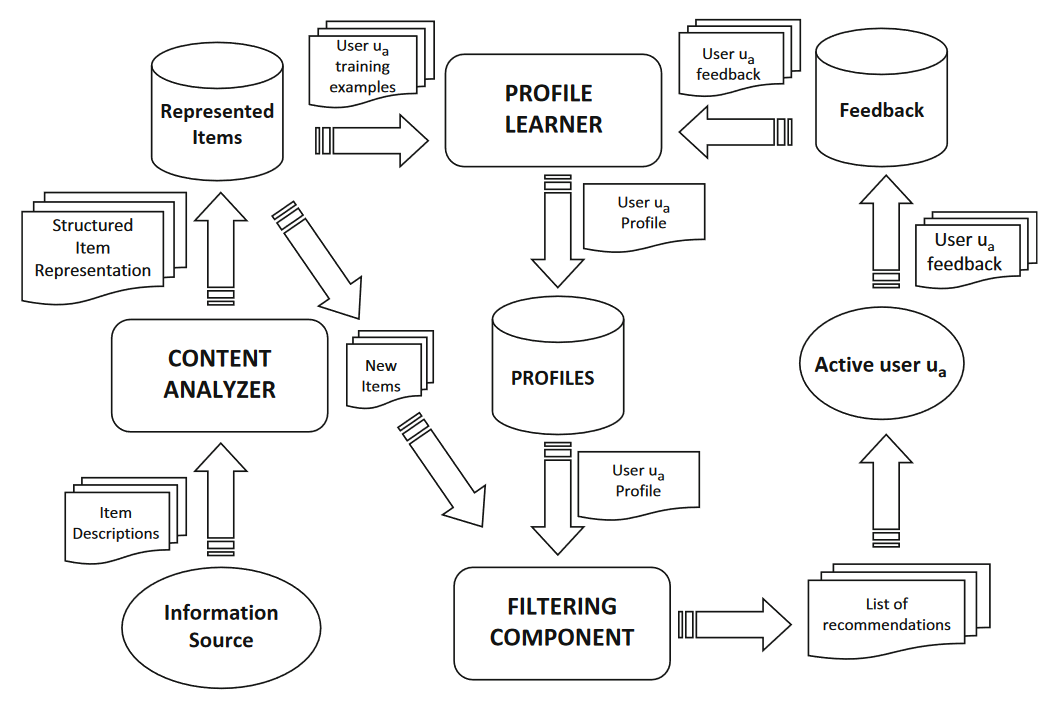
\includegraphics[width=0.6\textwidth]{img/content_based_figure_1.png}
    \caption{High level architecture of a content-based recommender \cite{Musto2022251}}
    \label{fig:high_lvl_content_based}
    \Description{It shows how user profiles are built using past interactions and item representations, and how these profiles are matched with new items to generate personalized recommendations.}
\end{figure}
%
\item \textbf{Collaborative Filtering:} Instead of analyzing item features, collaborative filtering leverages patterns in user-item interactions (e.g., ratings, clicks, purchases) to identify similar users or items. The two primary subtypes are user-based and item-based filtering. User-based filtering recommends items that like-minded users have enjoyed, while item-based filtering finds items that are often co-preferred \ref{fig:collaborative}. This method is effective for capturing complex user behavior without needing content metadata. However, it requires sufficient interaction data and typically struggles with the cold-start problem for new users or items \cite{NILASHI2018507}.
%
\begin{figure}[h]
  \centering
  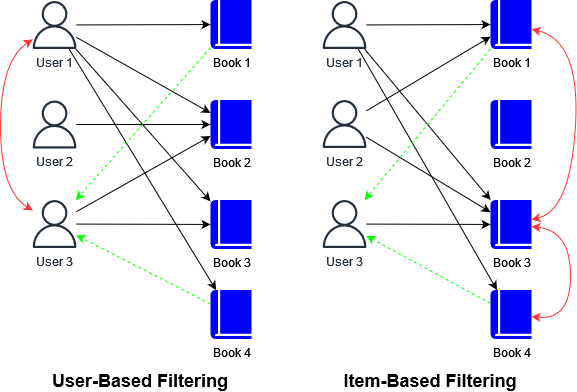
\includegraphics[width=0.6\linewidth]{img/collaborative_example.png}
  \caption{Illustration of Memory-based CF recommendation}
  \label{fig:collaborative}
  \Description{On the left, User-Based Filtering identifies users with similar preferences and recommends items they have liked to the active user. On the right, Item-Based Filtering finds items similar to those the active user has already rated or consumed, and recommends them based on item similarity.}
\end{figure}
%
\item \textbf{Context-Aware Approaches:} Contextual recommendation enhances traditional models by adding situational variables such as time of day, location, device used or user mood. This enables more adaptive and relevant suggestions. For instance, a travel app might prioritize warm destinations in winter or suggest restaurants near the user’s current GPS location. Context can be explicit (manually provided) or implicit (inferred from usage patterns)\cite{Haruna2017}.
%
\item \textbf{Knowledge Graph-Based Methods:} Knowledge graphs represent entities (items, authors, topics) and their relationships in a structured graph format. Recommender systems can traverse these graphs to discover paths and infer user-item relevance based on semantic proximity \ref{fig:knowledge_graph}. These approaches are particularly valuable in domains with rich metadata or ontologies—such as academic libraries or product catalogs—enabling explainable and diverse recommendations. Graph embeddings or path-based reasoning techniques (e.g., TransE, path ranking) are commonly employed to model semantic similarity \cite{Imene2022488}.
%
\begin{figure}[h]
	\centering
	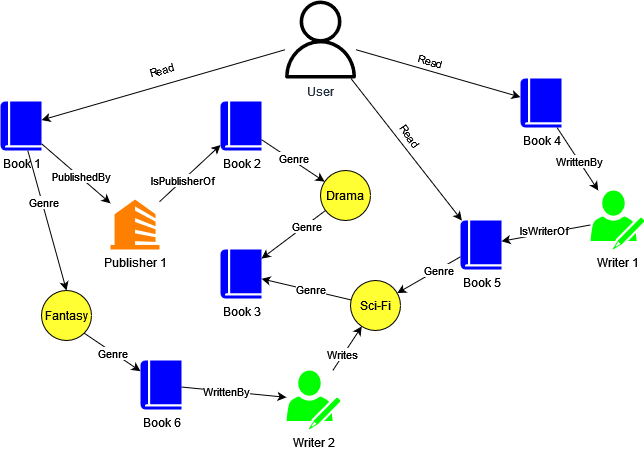
\includegraphics[width=0.6\linewidth]{img/knowledge_graph_example.png}
	\caption{Illustration of KG-aware recommendation}
	\label{fig:knowledge_graph}
\Description{It shows how entities such as books, genres, authors, and publishers are interconnected through semantic relationships (e.g., WrittenBy, Genre, PublishedBy).}
\end{figure}
%
\item \textbf{Popularity-Based Models:} These systems recommend items that are globally popular or trending across the user base. They are simple, highly scalable, and often used as default or fallback strategies, especially in the absence of personalization data. While effective in surfacing mainstream content, they ignore individual preferences and may use popularity bias by continually recommending  well-known items.

\item \textbf{Demographic-Based Filtering:} This method relies on user segmentation based on demographic attributes such as age, gender, location, or occupation. Recommendations are generated by identifying patterns or preferences within each group. For example, a platform might recommend young adult fiction to teenage readers or technical manuals to engineering professionals. Though useful in scenarios with limited interaction data, this approach risks stereotyping users and often lacks personalization depth \cite{Burke2002331}.

\item \textbf{Utility-Based Models:} Utility-based systems estimate the subjective value or utility of items for a user, often combining multiple criteria—such as cost, quality, and relevance—into a scoring function. These models are decision-theoretic in nature and are well-suited to domains where user decisions depend on multi-attribute trade-offs, such as travel booking or product selection scenarios. The main challenge is defining appropriate utility functions that reflect diverse user preferences \cite{Burke2002331}.

\item \textbf{Deep Learning-Based Methods:} Deep learning models offer powerful means for capturing intricate, non-linear patterns in user behavior and item characteristics. Architectures such as convolutional neural networks (CNNs), recurrent neural networks (RNNs), transformers, and autoencoders have been applied to recommendation tasks. These methods can process rich inputs such as text, images, or sequences of user interactions. While often achieving state-of-the-art performance, they typically require large-scale data and substantial computational resources for training and inference.

\item \textbf{Hybrid Approaches:} Hybrid systems combine two or more of the aforementioned techniques to leverage their complementary strengths. Common combinations include blending collaborative filtering with content-based filtering, or incorporating knowledge graphs into deep learning models. Strategies for hybridization include weighted ensembles, cascading (where one model filters candidates for another), or feature augmentation (where the output of one model becomes input for another). Hybrid models are often more robust, especially in complex recommendation scenarios involving cold-start users, sparse data, or diverse content types.
\end{itemize}


\subsection{System Roles and Stakeholder Objectives}
The role of a recommender system varies depending on whether it is viewed from the perspective of the service provider or the end-user. For example, a music streaming platform may use RS to boost user engagement, thereby increasing subscriptions or ad revenue, while the user simply seeks enjoyable or novel content.

From the provider’s perspective, common goals include:
\begin{itemize}
\item Increasing sales through cross-selling and upselling strategies,
\item Promoting less popular or long-tail items,
\item Enhancing overall user satisfaction and retention,
\item Gaining insights into user preferences to improve inventory management or marketing campaigns \cite{pub.1036183961}.
\end{itemize}

From the user’s standpoint, recommender systems assist with:
\begin{itemize}
    \item Discovering high-quality or relevant items,
    \item Browsing unfamiliar content with minimal effort,
    \item Exploring item bundles or sequences (e.g., course modules, book series),
    \item Understanding recommendations through contextual cues,
    \item Sharing opinions and assisting other users via feedback,
    \item Evaluating the system's credibility and refining their own profiles \cite{Ricci20221}.
\end{itemize}
%
By aligning system functionality with both user experience and business strategy, recommender systems continue to evolve as important tools across numerous digital platforms.
%
\subsection{Challenges in Recommendation Systems}
%
Despite their widespread use and effectiveness, recommendation systems face several critical challenges that affect their performance, accuracy, and user satisfaction. These challenges arise due to the complex and dynamic nature of user behavior, data limitations, and system constraints. Below are some of the most significant difficulties encountered across various types of recommendation systems:
%
\begin{itemize}
\item \textbf{Cold-Start Problem:}
One of the most common and well-documented issues is the cold-start problem, which occurs when a system must generate recommendations for new users or new items that have little to no historical data. Since most recommendation algorithms rely on past interactions to make predictions, this lack of data can lead to poor or irrelevant suggestions. Solutions often involve hybrid methods that incorporate content-based or demographic data to address the information gap \cite{Al-Hassan2024a}.
%
\item \textbf{Data Sparsity:}
In systems with a vast number of users and items, the user-item interaction matrix—used for collaborative filtering—is typically very sparse. This means that only a small fraction of possible interactions are known, making it difficult to identify patterns or similarities. Data sparsity reduces the effectiveness of similarity-based methods and can degrade overall recommendation accuracy.
%
\item \textbf{Scalability:}
As recommendation platforms grow to serve millions of users and items, scalability becomes a major concern. Algorithms must be designed to handle large-scale data efficiently, both in terms of computation and memory. Real-time recommendations further increase the demand for scalable, fast-performing systems.
%
\item \textbf{Diversity:}
Providing a diverse set of recommendations is important for user engagement and product discovery. However, some algorithms tend to recommend only highly similar or popular items, leading to a lack of novelty. This "filter bubble" effect can reduce user satisfaction over time. On the other hand, increasing diversity too aggressively may reduce relevance or precision, creating a trade-off that must be balanced carefully \cite{pub.1072601078}.
%
\item \textbf{Privacy Concerns:}
Personalized recommendations typically require collecting user data such as browsing history, preferences, or even location. While this data enhances prediction quality, it also raises privacy concerns. Users may feel uneasy or distrustful if the system appears to know too much about them, especially when data handling practices are not transparent. Ensuring data protection through anonymization and responsible data use is essential.
%
\item \textbf{Serendipity:}
Serendipity refers to the ability of a system to surprise users with unexpected but interesting recommendations. While this can enhance user experience, it must be balanced carefully. If too many recommendations are serendipitous and lack clear relevance, users might perceive the system as random or unreliable. A good recommender system must strike a balance between expected results and delightful surprises \cite{Aymen2022896}.
%
% \item \textbf{Exploration vs. Exploitation:}
% (Optional - not currently included)
\end{itemize}
These challenges highlight the need for continued innovation in algorithm design, evaluation methods, and user experience optimization. Addressing them effectively requires a combination of advanced techniques, domain-specific adaptations, and a deep understanding of user needs.






\section{Experimental Framework for Book Recommendation Systems}

To bridge the gap between theoretical foundations and practical application, this section outlines the framework developed to evaluate content-based recommendation systems on digital library datasets. The proposed framework supports a comparative analysis of multiple text representation algorithms and enables systematic experimentation and benchmarking, including preprocessing, model implementation and evaluation methodology.

The primary reason for selecting a content-based filtering approach in this work comes from the characteristics of the datasets involved. The evaluation in this work is based on two distinct datasets: one composed of academic book content segmented at the paragraph level, and another consisting of Goodreads entries containing short textual summaries of general fiction and non-fiction books. Both datasets focus exclusively on short-form text—paragraphs and summaries—rather than full documents. The academic dataset does not contain any form of user feedback or interaction data, making it unsuitable for collaborative filtering approaches that rely on user-item behavior. While the Goodreads dataset includes some aggregated feedback such as average ratings and number of reviews, it lacks any user-specific interaction history or behavioral traces. Because collaborative filtering techniques require explicit or implicit user-level feedback (e.g., clicks, ratings, co-consumption), they are not feasible in this scenario. For this reason, a content-based filtering approach was adopted, as it relies solely on the textual attributes of items and is well-suited for domains where user data is limited or unavailable.

To enable such content-based recommendations, a range of text representation models were selected, each offering a different level of linguistic or semantic abstraction. This diversity ensures that the evaluation captures performance variations across models that range from shallow frequency-based techniques to deep, contextual embeddings. Classical models like TF-IDF and Bag-of-Words provide interpretable and efficient baselines, capturing the statistical importance of terms within documents. Latent Semantic Analysis was included to explore the benefits of dimensionality reduction in uncovering hidden thematic relationships. Meanwhile, word embedding methods such as GloVe and FastText introduce pretrained semantic spaces that better capture word similarity and context independence, with FastText extending this to subword structures for handling rare terms. Finally, deep transformer-based encoders like BERT and E5 were integrated to evaluate the value of contextual understanding, where sentence-level meaning significantly influences recommendations.

The datasets were preprocessed using standard natural language techniques, including lowercasing, tokenization, and removal of punctuation and stopwords. Paragraphs and summaries were represented as fixed-length vectors using the chosen models, and recommendations were generated by computing cosine similarity between the input text and the candidate corpus. This vector-based similarity approach allowed for consistent comparison across models.

The evaluation was conducted through offline experiments and focused on measuring key system-centric metrics such as similarity, coverage, confidence, and diversity, as well as resource consumption. By combining multiple representation techniques with a unified recommendation pipeline, the framework not only enables reproducible benchmarking but also illustrates how the richness and type of text representation influence the effectiveness of recommendations when user data is absent.


%\section{Experimental Framework for Book Recommendation Systems}
%To bridge the gap between theoretical foundations and practical application, this section outlines the framework developed to evaluate content-based recommendation systems on digital library datasets. The proposed framework supports a comparative analysis of multiple text representation algorithms and enables systematic experimentation and benchmarking. It includes preprocessing, model implementation, evaluation methodology, and deployment architecture.
%
%\subsection{Dataset and Preprocessing}
%Two different datasets were used to ensure the system is tested across diverse domains:
%\begin{itemize}
%\item \textbf{Academic Book Paragraphs:} Extracted from digital libraries and stored in structured JSON format. Each entry corresponds to a paragraph, with metadata including book title, index, and location in the document.
%\item \textbf{Goodreads Descriptions:} A publicly available dataset containing metadata and short descriptions for a wide range of fiction and non-fiction books.
%\end{itemize}
%
%Before applying any text representation model, a preprocessing phase is performed to normalize and prepare the text data. The preprocessing pipeline includes:
%\begin{enumerate}
%    \item \textbf{Lowercasing:} All text is converted to lowercase to ensure uniformity.
%    \item \textbf{Tokenization:} Sentences are split into individual tokens (words or subwords).
%    \item \textbf{Punctuation and Special Character Removal:} Non-alphanumeric characters are filtered out to reduce noise.
%    \item \textbf{Stopword Removal:} Common words (e.g., “and”, “the”, “is”) that do not contribute to meaning are removed.
%    \item \textbf{Optional Stemming/Lemmatization:} Words are reduced to their root forms, depending on the representation method used.
%\end{enumerate}
%
%\subsection{Text Representation Models}
%Seven diverse models were chosen to represent book text, ranging from classical statistical to advanced neural network-based approaches:
%\begin{itemize}
%    \item TF-IDF
%    \item Bag-of-Words (BoW)
%    \item Latent Semantic Analysis (LSA)
%    \item GloVe
%    \item FastText
%    \item BERT (SentenceTransformer)
%    \item E5 (Embedding-based Encoder for Retrieval)
%\end{itemize}
%
%Each model captures different linguistic features and levels of semantic abstraction, allowing the framework to measure their effectiveness under varying conditions.
%
%\subsection{Recommendation Pipeline}
%The system follows a modular pipeline architecture with a shared interface for all models:
%\begin{enumerate}
%    \item \textbf{Model Initialization:} Load or train the selected model.
%    \item \textbf{Text Vectorization:} Transform input texts into vector form using the selected model.
%    \item \textbf{Similarity Computation:} Use cosine similarity to compute pairwise similarity between vectors.
%    \item \textbf{Filtering and Ranking:} Apply thresholds and sort top-N recommendations.
%    \item \textbf{Output Storage:} Save results with metadata and resource tracking (CPU, GPU, memory).
%\end{enumerate}
%
%\subsection{Evaluation Strategy}
%The evaluation focuses on \textbf{offline experiments}, which simulate user behavior without requiring real-time interaction. Key metrics include:
%\begin{itemize}
%    \item \textbf{Similarity:} How well the recommended items align with the input.
%    \item \textbf{Coverage:} Proportion of items receiving a recommendation.
%    \item \textbf{Diversity:} How varied the recommended items are.
%    \item \textbf{Confidence:} Strength of similarity scores among recommended items.
%    \item \textbf{Resource Usage:} Time and memory cost of each algorithm.
%\end{itemize}
%

%\subsection{Benefits of the Framework}
%The framework enables:
%\begin{itemize}
%    \item \textbf{Consistent Evaluation:} All models use the same recommendation logic and metrics.
%    \item \textbf{Extensibility:} New models can be integrated with minimal configuration.
%    \item \textbf{Domain Versatility:} Datasets span academic and popular literature domains.
%    \item \textbf{Reproducibility:} Each experiment is repeatable and transparently logged.
%\end{itemize}
%
%This comprehensive evaluation environment offers practical insights into the performance of various content-based recommendation approaches, highlighting the trade-offs in recommendation quality, diversity, and efficiency across datasets and algorithms.


\section{Evaluation of Recommender Systems}

Recommendation algorithms can be evaluated using various metrics depending on the system’s intended purpose and available data. Evaluation methods are broadly classified into two categories: \textbf{system-centric} and \textbf{user-centric} evaluations \cite{Zangerle2023, Gunawardana2022547}.

\begin{itemize}
    \item \textbf{System-Centric Evaluation} examines the algorithm's internal performance, using quantitative metrics such as similarity, diversity, and coverage. It is suitable for offline experiments and content-based evaluation.
    \item \textbf{User-Centric Evaluation} involves interaction studies (e.g., surveys, A/B tests) to assess user satisfaction, perceived quality, and usability.
\end{itemize}

In scenarios where user-item interaction data is unavailable—such as digital libraries or offline textual datasets—traditional metrics like precision or recall are not applicable. In these cases, system-centric evaluation enables performance benchmarking using metrics derived from content similarity and catalog structure.

\subsubsection{Overview of Evaluation Metrics}

Table~\ref{tab:eval-metrics} provides a consolidated view of recommendation metrics, grouped by purpose and annotated with their data requirements. This overview informs the rationale for the specific evaluation strategy used in this work.

\begin{table}[H]
\caption{Overview of Recommendation Evaluation Metrics}
\label{tab:eval-metrics}
\begin{tabular}{p{0.22\linewidth}p{0.58\linewidth}p{0.16\linewidth}}
\toprule
\textbf{Metric Category} & \textbf{Description} & \textbf{Requires User Feedback?} \\
\midrule
\textbf{Rating Accuracy} & Measures the difference between predicted and true user ratings (e.g., RMSE, MAE) & Yes \\
\textbf{Usage Prediction} & Measures success in recommending used items (e.g., Precision, Recall, F1, AUC) & Yes \\
\textbf{Ranking Quality} & Evaluates ordering of relevant items (e.g., NDCG, MRR, ARHR, Spearman's $\rho$) & Yes \\
\textbf{Similarity} & Measures cosine similarity between input and recommended items & No \\
\textbf{Diversity} & Captures dissimilarity among recommended items (via score variance or pairwise distance) & No \\
\textbf{Confidence} & Reflects consistency in similarity scores across top-N recommendations & No \\
\textbf{Coverage} & Proportion of catalog items that are recommended at least once & No \\
\textbf{Novelty} & Degree to which recommended items are unfamiliar to users (e.g., based on popularity thresholds) & Partial \\
\textbf{Popularity} & Proportion of well-known or high-rating items in the recommendations & Partial \\
\textbf{Serendipity} & Surprise factor—items both unexpected and useful to the user & Yes \\
\textbf{Trust} & Perceived credibility and reliability of recommendations & Yes \\
\textbf{Utility} & Value of recommended items to the user in practical scenarios & Yes \\
\textbf{Scalability} & Ability of the system to perform under growing data volume & No \\
\textbf{Robustness} & Resistance to noise or malicious input & No \\
\textbf{Privacy} & Ability to preserve user anonymity or minimize data exposure & No \\
\textbf{Risk} & Cost or danger of a wrong recommendation (e.g., in healthcare) & Yes \\
\textbf{Adaptability} & System’s responsiveness to changes in user behavior or data & Yes \\
\bottomrule
\end{tabular}
\end{table}

\subsubsection{Selected Metrics for This Study}

Due to the lack of user-specific interaction data in the datasets used (academic paragraphs and Goodreads summaries without user histories), this study adopts a \textbf{system-centric} and \textbf{content-level} evaluation strategy. The goal is to analyze the structural quality of the top-N recommendations produced by different text representation models.

The following metrics were selected and computed based on top-10 recommendations per input item:

\begin{itemize}
    \item \textbf{Similarity:} Measures the average cosine similarity between the input and recommended items. A higher score indicates semantic closeness.

    \item \textbf{Diversity:} Quantifies the range of content in recommendations using:
    \begin{itemize}
        \item \textit{Similarity Variance:} Variance among similarity scores.
        \item \textit{Pairwise Dissimilarity:} Average of \(1 - \text{cosine similarity}\) across pairs.
    \end{itemize}
    Higher diversity increases the recommendation breadth and avoids redundancy \cite{Silveira2019813}.

    \item \textbf{Confidence:} Indicates stability of recommendations, calculated as:
    \begin{equation}
    \label{eq:confidence}
    \text{Confidence} = \frac{1}{1 + \text{std\_dev(similarities)}}
    \end{equation}
    A lower standard deviation in similarity values leads to higher confidence.

    \item \textbf{Coverage:} Assesses how many unique items from the dataset appear in recommendations. A dynamic similarity threshold—based on model-specific behavior—was applied to filter out weak matches.

    \item \textbf{Novelty:} Measures exposure to lesser-known items. Recommendations falling below the 25th percentile in rating, rating count, and review count were classified as novel \cite{Avazpour2014245}.

    \item \textbf{Popularity:} Evaluates the tendency to recommend mainstream items. Items exceeding dataset averages for rating and in the top quartile for review metrics were labeled popular.
\end{itemize}

These metrics were chosen for their ability to capture both the quality and the variety of content-based recommendations, especially in domains like digital libraries where personalization data is often sparse. They collectively offer insight into the semantic relevance, range, and uniqueness of each model’s outputs, as well as their computational and practical applicability \cite{De_Nart201484}.

%\section{Evaluation and Results}
%
%This section presents the evaluation methodology used to assess the performance of various content-based recommendation algorithms and summarizes the experimental results. A robust evaluation is essential to determine which techniques best serve a given recommendation context, particularly when user feedback is unavailable. In this study, we designed an offline, system-centric evaluation strategy tailored to short-text digital book datasets.
%
%\subsection{Evaluation of Recommender Systems}
%
%Recommendation algorithms can be assessed from different perspectives depending on the intended use case. Broadly, evaluation strategies fall into two main categories: \textbf{system-centric} and \textbf{user-centric} evaluations \cite{Zangerle2023}. 
%
%\begin{itemize}
%    \item \textbf{System-Centric Evaluation} focuses on the algorithmic performance of the recommendation engine. It includes measures such as accuracy, similarity, diversity, and computational efficiency. These metrics are typically derived from the content or structure of the data and are well suited to offline experiments.
%    \item \textbf{User-Centric Evaluation} involves user studies, A/B testing, or surveys to gauge how users perceive and interact with the recommendations. It considers usability, satisfaction, and subjective quality.
%\end{itemize}
%
%This study adopts a system-centric evaluation approach due to the absence of interaction data. Most traditional metrics such as precision, recall, NDCG, and user ranking correlation require user-level feedback or interaction logs. These were not available in our datasets. Thus, we relied on internal content-based metrics such as similarity, diversity, confidence, coverage, popularity, and novelty.
%
%Beyond accuracy, recommender systems should also account for qualitative aspects such as diversity, novelty, and system scalability. This is particularly important in domains like academic and digital libraries where user populations are smaller, preferences are dynamic, and implicit feedback is scarce \cite{De_Nart201484, Gunawardana2022547}. Content-based filtering is especially well-suited to such domains due to its ability to operate solely on item metadata without relying on large-scale user activity.
%%
%\subsection{Evaluation Metrics and Rationale}
%The evaluation metrics were designed to compare text representation methods in terms of the quality and characteristics of their recommendations. All metrics are computed over the top-10 recommendations per input item, focusing on the most relevant outputs while maintaining interpretability. The selected metrics are: \cite{Gunawardana2022547}
%%
%\begin{itemize}
%    \item \textbf{Similarity:} Measures the average cosine similarity between the input item and the recommended items. It reflects how closely related the items are based on textual representation.
%    
%    \item \textbf{Diversity:} Captures the degree of variation among recommended items. Two methods were applied:
%        \begin{itemize}
%            \item Variance of similarity scores among the recommendations.
%            \item Average pairwise dissimilarity (\(1 - \text{cosine similarity}\)) among the top recommendations.
%        \end{itemize}
%    Higher diversity prevents redundancy and increases the likelihood of covering broader topics \cite{Silveira2019813}.
%
%\item \textbf{Confidence:} Indicates how consistent the similarity scores are across the recommendations. Calculated as the inverse of the standard deviation of similarity scores, shown in Equation~\ref{eq:confidence}. A higher confidence score reflects more stable and trustworthy recommendations.
%\begin{equation}
%\label{eq:confidence}
%\text{Confidence} = \frac{1}{1 + \text{std\_dev(similarities)}}
%\end{equation}
%
%    \item \textbf{Coverage:} Measures the proportion of unique items recommended across all input queries, relative to the size of the dataset. A higher coverage indicates broader use of the item catalog. A dynamic similarity threshold was applied to filter weak matches, tailored per model type based on empirical analysis.
%
%    \item \textbf{Novelty:} Assesses how likely it is that the recommended items are unknown to the average user. Recommendations were labeled as novel if they scored below the 25th percentile for rating, rating count, and review count based on Goodreads metadata \cite{Avazpour2014245}.
%
%    \item \textbf{Popularity:} The opposite of novelty. An item was marked as popular if it exceeded the average rating and was above the 75th percentile in both rating and review count.
%\end{itemize}
%
%These metrics provide a balanced view of relevance, reach, surprise, and system-level behavior.

%\begin{figure}[H]
%	\centering
%	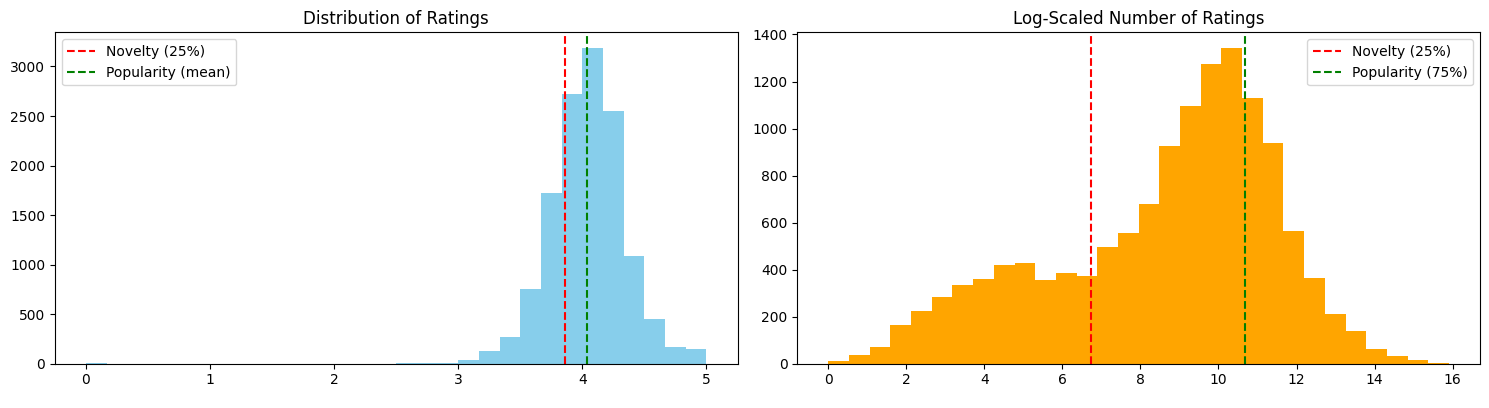
\includegraphics[width=\linewidth,keepaspectratio]{img/ratings_novelty_popularity2.png}
%	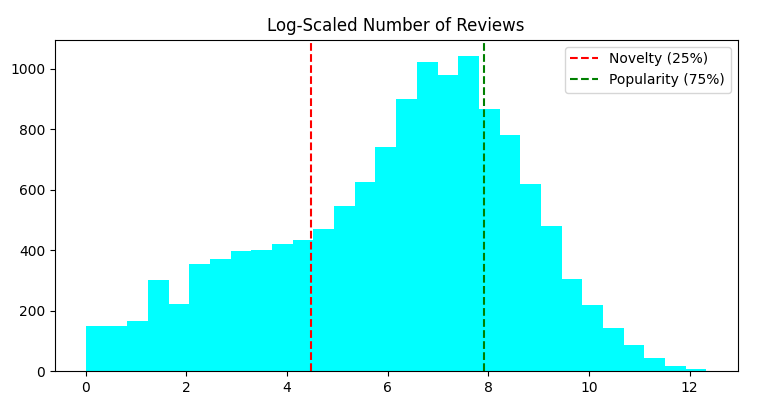
\includegraphics[width=\dimexpr0.5\linewidth\relax,keepaspectratio]{img/ratings_novelty_popularity3.png}
%	\caption{Distribution of ratings and reviews in Goodreads dataset}
%	\label{fig:ratings_chart}
%\end{figure}

\subsection{Results on Book Descriptions}

Figure~\ref{fig:descriptions_radar} visualizes each algorithm’s normalized performance across the evaluation metrics for the Goodreads book description dataset.

\begin{figure}[h!]
    \centering
    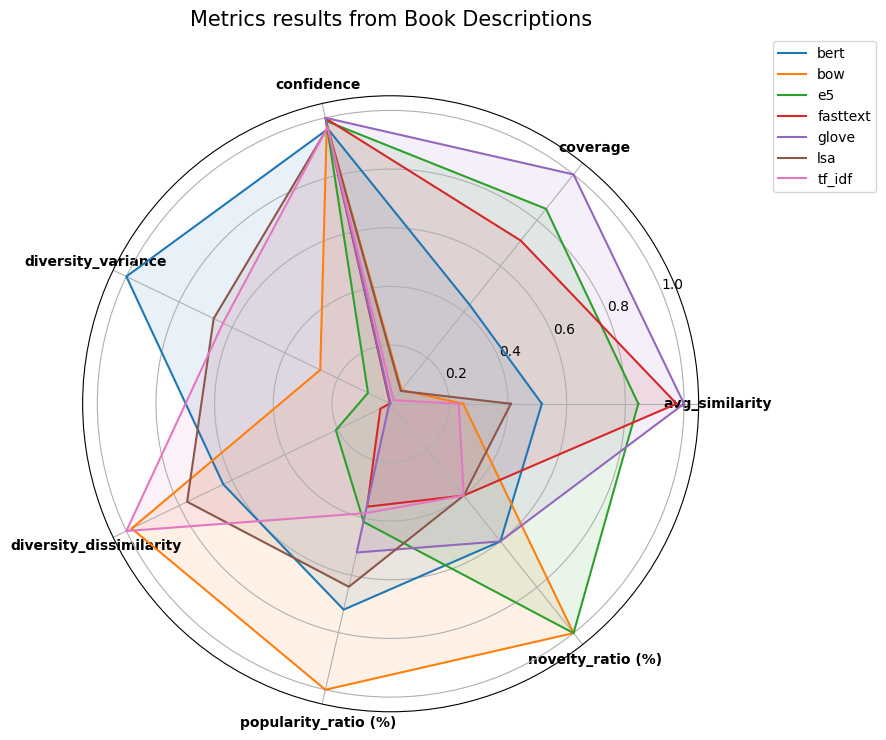
\includegraphics[width=0.8\linewidth,keepaspectratio]{img/descriptions_metrics_radar2.png}
    \caption{Metrics Results of Descriptions Visualized}
    \label{fig:descriptions_radar}
\end{figure}

\noindent Key observations from the results:
\begin{itemize}
    \item \textbf{FastText}, \textbf{E5}, and \textbf{GloVe} led in \textbf{coverage} and \textbf{confidence}, suggesting robust recommendations across a wide item range.
    \item \textbf{BERT} showed highest variance in diversity, while \textbf{BoW} and \textbf{TF-IDF} excelled in dissimilarity-based diversity.
    \item \textbf{BoW} and \textbf{E5} achieved top scores in both \textbf{popularity} and \textbf{novelty}, indicating an ability to surface both mainstream and niche items.
\end{itemize}

%\begin{table}[H]
%\centering
%\large
%\begin{tabular}{|l|c|c|c|c|c|c|c|}
%\hline
%\textbf{Model} & \textbf{Sim} & \textbf{Cov} & \textbf{Conf} & \textbf{Div (Var.)} & \textbf{Div (Diss.)} & \textbf{Pop (\%)} & \textbf{Nov (\%)} \\
%\hline
%bert     & 0.513 & 9.29  & 0.96039 & 0.00223 & 0.4866 & 18.00 & 3.00 \\
%bow      & 0.246 & 1.29  & 0.97755 & 0.00059 & 0.7530 & 25.00 & 5.00 \\
%e5 		& 0.840 & 18.29 & 0.98830 & 0.00019 & 0.1593 & 10.33 & 5.00 \\
%fasttext & 0.970 & 15.31 & 0.99765 & 0.00001 & 0.0299 & 9.00  & 2.00 \\
%glove    & 0.995 & 21.52 & 0.99946 & 0.00000 & 0.0045 & 13.00 & 3.00 \\
%lsa      & 0.408 & 1.20  & 0.96473 & 0.00149 & 0.5917 & 16.00 & 2.00 \\
%tf\_idf  & 0.231 & 0.34  & 0.96648 & 0.00141 & 0.7684 & 9.56  & 2.00 \\
%\hline
%\end{tabular}
%\caption{Results of Metrics for Book Descriptions}
%\label{tab:metrics_desc}
%\end{table}

%\begin{table}[H]
%\centering
%\begin{tabular}{lccc}
%\textbf{Algorithm} & \textbf{CPU Time (s)} & \textbf{RAM (MB)} & \textbf{GPU Mem (MB)} \\
%\hline
%BERT     & 27.76 & 1141.38 & 563.78 \\
%E5       & 106.78 & 1200.35 & 1732.01 \\
%BoW      & 0.28  & 202.89  & - \\
%FastText & 11.82 & 1193.43 & - \\
%GloVe    & 3.21  & 344.33  & - \\
%LSA      & 2.04  & 424.85  & - \\
%TF-IDF   & 1.73  & 193.64  & - \\
%\end{tabular}
%\caption{Average Resource Usage for Book Description Recommendations}
%\label{tab:performance-desc}
%\end{table}

\subsection{Results on Academic Paragraphs}

Figure~\ref{fig:paragraphs_radar} summarizes the evaluation of models on paragraph-level academic book data.

\begin{figure}[h!]
    \centering
    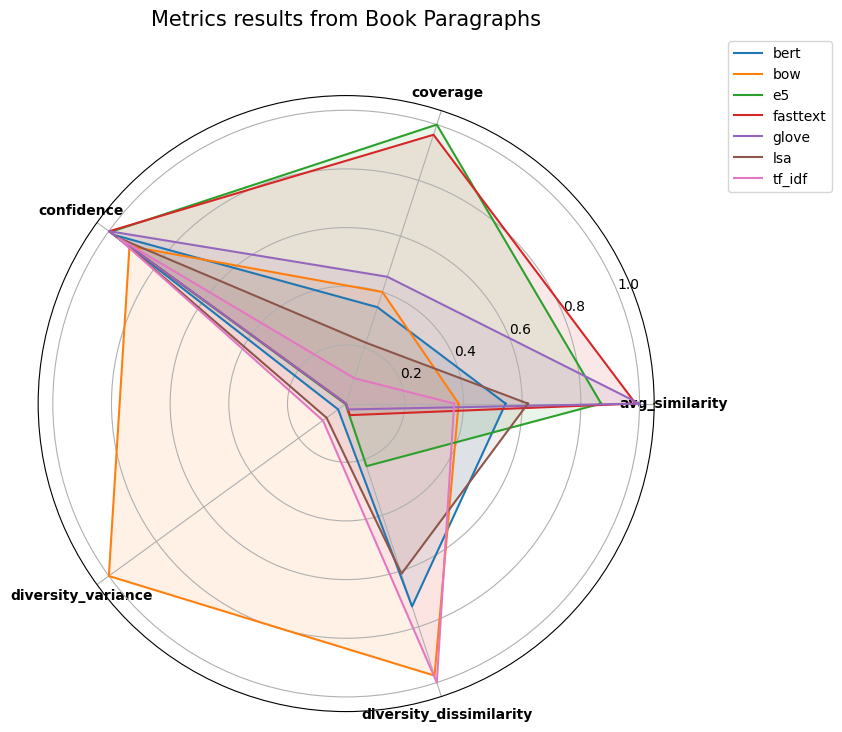
\includegraphics[width=0.8\linewidth,keepaspectratio]{img/paragraphs_metrics_radar2.png}
    \caption{Metrics Results of Paragraphs Visualized}
    \label{fig:paragraphs_radar}
\end{figure}

\noindent Key observations:
\begin{itemize}
    \item \textbf{GloVe}, \textbf{FastText}, and \textbf{E5} scored highest in \textbf{similarity} and \textbf{coverage}, capturing semantic meaning effectively.
    \item \textbf{BoW} and \textbf{TF-IDF} again delivered strong results in diversity, showing their ability to produce heterogeneous recommendations.
    \item All models had consistently high confidence, indicating stable performance even in more technical or domain-specific content.
\end{itemize}

%\begin{table}[h!]
%\centering
%\large
%\begin{tabular}{|l|c|c|c|c|c|}
%\hline
%\textbf{Model} & \textbf{Sim} & \textbf{Cov} & \textbf{Conf} & \textbf{Div (Var.)} & \textbf{Div (Diss.)} \\
%\hline
%bert     & 0.536 & 0.19 & 0.97654 & 0.00060  & 0.463  \\
%bow      & 0.378 & 0.22 & 0.91190 & 0.01781  & 0.621  \\
%e5		& 0.857 & 0.55 & 0.99352 & 0.00005  & 0.143 \\
%fasttext & 0.973 & 0.53 & 0.99791 & 0.00001  & 0.026 \\
%glove    & 0.986 & 0.25 & 0.99877 & 0.00000  & 0.013 \\
%lsa      & 0.611 & 0.12 & 0.96231 & 0.00147  & 0.389 \\
%tf\_idf  & 0.363 & 0.05 & 0.95945 & 0.00174  & 0.637 \\
%\hline
%\end{tabular}
%\caption{Results of Metrics for Book Paragraphs}
%\label{tab:metrics_para}
%\end{table}

%\begin{table}[H]
%\centering
%\begin{tabular}{lccc}
%\textbf{Algorithm} & \textbf{CPU Time (s)} & \textbf{RAM (MB)} & \textbf{GPU Mem (MB)} \\
%\hline
%BERT     & 103.40 & 1227.44 & 670.89 \\
%E5       & 482.16 & 1313.28 & 1824.20 \\
%BoW      & 0.81   & 378.45  & - \\
%FastText & 44.96  & 2002.80 & - \\
%GloVe    & 10.31  & 420.78  & - \\
%LSA      & 8.18   & 744.64  & - \\
%TF-IDF   & 7.23   & 293.49  & - \\
%\end{tabular}
%\caption{Average Resource Usage for Book Paragraph Recommendations}
%\label{tab:performance-paragraph}
%\end{table}



\section{Conclusion}

This study investigated the effectiveness of various content-based recommendation algorithms applied to digital library datasets, with a focus on textual representations. Two distinct datasets were employed: one derived from academic book paragraphs and another from Goodreads, containing book summaries and associated metadata. The experimental framework compared seven text representation methods—\textit{TF-IDF}, \textit{BoW}, \textit{LSA}, \textit{GloVe}, \textit{FastText}, \textit{BERT}, and \textbf{E5}—using cosine similarity to generate recommendations.

A system-centric evaluation approach was adopted to ensure consistent and objective comparison. The metrics—similarity, diversity, confidence, coverage, novelty, and popularity—were chosen to assess the quality, stability, and variability of recommendations in the absence of user interaction data. In addition to recommendation quality, resource usage metrics such as execution time and memory consumption were evaluated to understand the computational trade-offs of each model.

The results demonstrated that dense embedding models such as \textit{GloVe}, \textit{E5}, and \textit{FastText} performed best in terms of similarity, coverage, and confidence, effectively identifying semantically relevant content. On the other hand, traditional models like \textit{BoW} and \textit{TF-IDF} produced higher diversity and unexpectedly achieved high scores in both popularity and novelty, likely due to their reliance on distinctive term overlaps. \textit{BERT} and \textit{E5} delivered strong overall performance but incurred higher computational costs.

Overall, the proposed evaluation framework enabled reproducible benchmarking of content-based recommenders, offering valuable insights into the trade-offs between semantic relevance, diversity, and efficiency. The methodology can be extended to other domains and datasets, supporting further research in content-aware recommendation systems.

\subsection{Future Work}

Several extensions could enhance the current framework and further explore the potential of recommendation systems in digital library contexts. Incorporating more recent state-of-the-art language models, especially transformer-based architectures, may improve semantic understanding and recommendation quality.

The evaluation could also be broadened by applying the framework to multilingual datasets, other media formats (e.g., abstracts, journal articles), or content from different domains such as education, healthcare, or entertainment. Improvements to text preprocessing—such as advanced normalization, domain-specific tokenization, or entity resolution—could further boost model performance.

Finally, while this study focused exclusively on content-based filtering due to the absence of user interaction data, future implementations may integrate collaborative or hybrid recommendation approaches. These would require user-level behavior data (e.g., clicks, ratings, session logs) to personalize and refine recommendations based on collective preferences. Exploring these dimensions would expand the framework’s applicability to more interactive and adaptive recommendation environments.



\bibliographystyle{ACM-Reference-Format}
%\bibliography{sample-base}
\bibliography{literature}



\end{document}
\endinput
